\definecolor{red}{rgb}{1,0,0}
\definecolor{green}{rgb}{0,0.39,0}
\renewcommand{\arraystretch}{1.1}

\subsection{Architecture}
\begin{frame}
\frametitle{VGG-16}
\framesubtitle{Architecture (2014)} 

\begin{textblock}{15}(7.67,-0.62)
	\begin{figure}[H]
		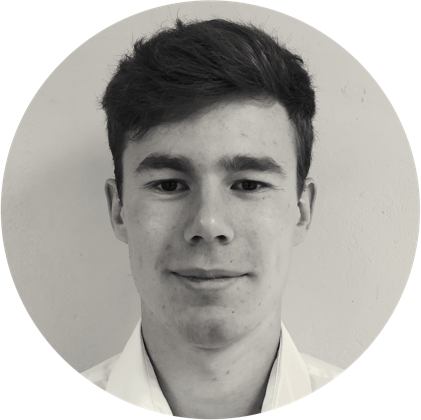
\includegraphics[width=0.1\textwidth]{Images/Team/DamienTOOMEY.png} 
	\end{figure}
\end{textblock}

\begin{textblock}{1}(8.35,1)
	\centerline{16 trainable layers ; 138,357,544 parameters}
\end{textblock}

\begin{center}

{\fontsize{8.5}{0}\selectfont
\begin{tabular}{ccccc}
\textbf{Layer} & \textbf{Type} & \textbf{Activation function} & \textbf{Output Shape} & \textbf{Param} \\
input\_1  & (\textcolor{gray}{InputLayer}) & N/A & (224, 224, 3) & \colorbox{yellow}{0} \\         
block1\_conv1 & (\textcolor{orange}{Conv2D}) & ReLU & (224, 224, 64) & 1,792 \\      
block1\_conv2 & (\textcolor{orange}{Conv2D}) & ReLU & (224, 224, 64) & 36,928 \\     
block1\_pool & (\textcolor{blue}{MaxPooling2D}) & N/A & (112, 112, 64) & \colorbox{yellow}{0} \\         
block2\_conv1 & (\textcolor{orange}{Conv2D}) & ReLU & (112, 112, 128) & 73,856 \\     
block2\_conv2 & (\textcolor{orange}{Conv2D}) & ReLU & (112, 112, 128) & 147,584 \\    
block2\_pool & (\textcolor{blue}{MaxPooling2D}) & N/A & (56, 56, 128) & \colorbox{yellow}{0} \\         
block3\_conv1 & (\textcolor{orange}{Conv2D}) & ReLU & (56, 56, 256) & 295,168 \\    
block3\_conv2 & (\textcolor{orange}{Conv2D}) & ReLU & (56, 56, 256) & 590,080 \\    
block3\_conv3 & (\textcolor{orange}{Conv2D}) & ReLU & (56, 56, 256) & 590,080 \\    
block3\_pool & (\textcolor{blue}{MaxPooling2D}) & N/A & (28, 28, 256) & \colorbox{yellow}{0} \\         
block4\_conv1 & (\textcolor{orange}{Conv2D}) & ReLU & (28, 28, 512) & 118,0160 \\   
block4\_conv2 & (\textcolor{orange}{Conv2D}) & ReLU & (28, 28, 512) & 2,359,808 \\   
block4\_conv3 & (\textcolor{orange}{Conv2D}) & ReLU & (28, 28, 512) & 2,35,9808 \\   
block4\_pool & (\textcolor{blue}{MaxPooling2D}) & N/A & (14, 14, 512) & \colorbox{yellow}{0} \\         
block5\_conv1 & (\textcolor{orange}{Conv2D}) & ReLU & (14, 14, 512) & 2,359,808 \\   
block5\_conv2 & (\textcolor{orange}{Conv2D}) & ReLU & (14, 14, 512) & 2,359,808 \\   
block5\_conv3 & (\textcolor{orange}{Conv2D}) & ReLU & (14, 14, 512) & 2,359,808 \\   
block5\_pool & (\textcolor{blue}{MaxPooling2D}) & N/A & (7, 7, 512) & \colorbox{yellow}{0} \\         
flatten & (Flatten) & N/A & (, 25088) & \colorbox{yellow}{0} \\         
fc1 & (\textcolor{green}{Dense}) & ReLU & (, 4096) & \colorbox{magenta}{102,764,544} \\ 
fc2 & (\textcolor{green}{Dense}) & ReLU & (, 4096) & 16,781,312 \\  
predictions & (\textcolor{green}{Dense}) & \textcolor{red}{Softmax} & (, 1000) & 4,097,000   
\end{tabular}
}
\end{center}
\end{frame}

\begin{frame}
\frametitle{VGG-16}
\framesubtitle{Transfer Learning} 

\begin{textblock}{15}(7.67,-0.62)
	\begin{figure}[H]
		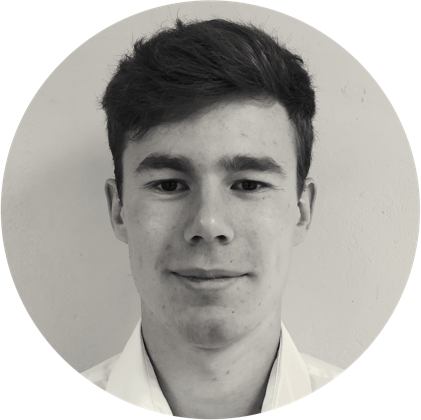
\includegraphics[width=0.1\textwidth]{Images/Team/DamienTOOMEY.png} 
	\end{figure}
\end{textblock}

\vspace{-0.7cm}
\begin{center}
{\fontsize{8.5}{8}\selectfont
\begin{tabular}{@{\hspace{-0.2cm}}cccc}
& \textbf{Layer Type} &\textbf{Activation function} & \textbf{Output Shape} \\
& & \textcolor{white}{phantom} & \\
	\begin{tabular}{c}
	freeze weights\\ learned on ImageNet
	\end{tabular}	
	& $\left\{\begin{tabular}{c}
	(\textcolor{gray}{InputLayer}) \\         
	(\textcolor{orange}{Conv2D}) \\      
	(\textcolor{orange}{Conv2D}) \\     
	(\textcolor{blue}{MaxPooling2D}) \\         
	(\textcolor{orange}{Conv2D}) \\     
	(\textcolor{orange}{Conv2D}) \\    
	(\textcolor{blue}{MaxPooling2D}) \\         
	(\textcolor{orange}{Conv2D}) \\    
	(\textcolor{orange}{Conv2D}) \\    
	(\textcolor{orange}{Conv2D}) \\    
	(\textcolor{blue}{MaxPooling2D}) \\         
	(\textcolor{orange}{Conv2D}) \\   
	(\textcolor{orange}{Conv2D}) \\   
	(\textcolor{orange}{Conv2D}) \\   
	(\textcolor{blue}{MaxPooling2D}) \\         
	(\textcolor{orange}{Conv2D}) \\   
	(\textcolor{orange}{Conv2D}) \\   
	(\textcolor{orange}{Conv2D})  \\   
	(\textcolor{blue}{MaxPooling2D})\\         
	(Flatten) \\         
	(\textcolor{green}{Dense}) \\ 
	(\textcolor{green}{Dense}) \\
	\end{tabular}
	\right.\kern-\nulldelimiterspace$
	& \begin{tabular}{c}
	N/A \\
	ReLU \\
	ReLU \\
	N/A \\
	ReLU \\
	ReLU \\
	N/A \\
	ReLU \\
	ReLU \\
	ReLU \\
	N/A \\
	ReLU \\
	ReLU \\
	ReLU \\
	N/A \\
	ReLU \\
	ReLU \\
	ReLU \\
	N/A \\
	N/A \\
	ReLU \\
	ReLU \\	
	\end{tabular}
	& \begin{tabular}{c}
	(224, 224, 3) \\
	(224, 224, 64) \\
	(224, 224, 64) \\
	(112, 112, 64) \\
	(112, 112, 128) \\
	(112, 112, 128) \\
	(56, 56, 128) \\
	(56, 56, 256) \\
	(56, 56, 256) \\
	(56, 56, 256) \\
	(28, 28, 256) \\ 
	(28, 28, 512) \\
	(28, 28, 512) \\
	(28, 28, 512) \\
	(14, 14, 512) \\
	(14, 14, 512) \\
	(14, 14, 512) \\
	(14, 14, 512) \\
	(7, 7, 512) \\
	(, 25088) \\
	(, 4096) \\
	(, 4096) \\
	\end{tabular} \\
	& \hspace{0.2cm} \sout{(\textcolor{green}{Dense})} & \sout{\textcolor{red}{Softmax}} & \sout{(, 1000)} \\
	\only<2>{& \hspace{0.2cm} \textcolor{magenta}{(Dropout)} & N/A & (, 4096) \\} 
	train this layer & \hspace{-0.5cm} $\left\{\begin{tabular}{c}
	\hspace{0.5cm} (\textcolor{green}{Dense})
	\end{tabular} \right.\kern-\nulldelimiterspace$ & \textcolor{red}{Softmax} & \hspace{0.1cm} (, nbClasses)
\end{tabular}
}
\end{center}

\end{frame}
